\section{Predictive Modeling}
\noindent
Using the processed data from \cref{section:exploratory_analysis}, I finally could start on designing a predictive model.

\subsection{Principal Component Analysis}
Even though I had majorly reduced the dimensionality of the data from 48 columns to only 12 columns through the processing steps, this was still too much data to pass into a predictive model. As a result, I decided to use Principal Component Analysis (PCA), which reduces data dimensionality while retaining most of the relevant information.

\noindent
\newline
PCA involves:
\begin{enumerate}
    \item Centering the data about the origin.
    \begin{itemize}
        \item \(X'_i = X_i - \bar{X}\)
    \end{itemize}
    \item Calculating the covariance matrix with n variables.
    \begin{itemize}
        \item \(Cov(X, Y) = \frac{1}{n-1} \sum_{i=1}^{n} \left(X'_i-\bar{X}\right) \left(Y'_i-\bar{Y}\right) \)
    \end{itemize}
    \item Compute the eigenvalues \(\lambda\) and eigenvectors \(v\) of the covariance matrix \(C\).
    \begin{itemize}
        \item \(Cv = \lambda v\)
    \end{itemize}
    \item Selecting the top \(k\) principal component eigenvalues and corresponding eigenvectors.
    \item Projecting an original point (X) onto the new feature space along the ith principle component \(v_i\).
    \begin{itemize}
        \item \(X' = X \dot v_i\)
    \end{itemize}
    \item The principal components are linear combinations of the original variables. \(a_{ij}\) represents the components of the ith eigenvector. This represents the general form for the principal component i.
    \begin{itemize}
        \item \(PC_i = a_{i1} X'_1 + a_{i2} X'_2 + \dots + a_{in} X'_n\)
    \end{itemize}
\end{enumerate}

\noindent
After performing PCA, the explained variance ratio can be derived using the Equation \ref{eq:explained_variance}. Using PC1, PC2, ..., and PC8, over 80\% of the variance in the accident severity is captured. This is described in the Scree Plot in \cref{fig:scree_plot}.

\begin{equation} \label{eq:explained_variance}
    \text{Explained Variance} = \frac{\lambda_i}{\lambda_1 + \lambda_2 + \dots +\lambda_n}
\end{equation}

\begin{figure}[H]
    \centering
    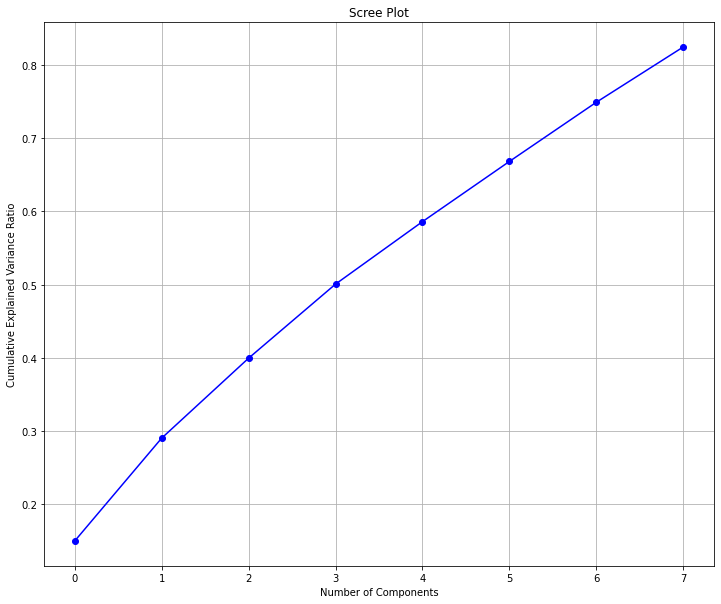
\includegraphics[width=100mm,height=\textheight,keepaspectratio]{images/scree_plot.png}
    \caption{Scree Plot}
    \label{fig:scree_plot}
\end{figure}

\subsection{Binary Logisitic Regression}
\label{section:logistic_regression}
In order to prevent overfitting and address the bias-variance tradeoff \citep{belkin2019reconciling}, I split the data into 80\% training and 20\% testing. Using the PCs derived in the previous step, I decided to try using a binary logistic regression.

\noindent
\newline
A binary logistic regression is defined by Equation \ref{eq:logistic_regression}.
\begin{equation} \label{eq:logistic_regression}
    y=\frac{1}{1+e^{-\left(\beta_0 + \beta_1 x \right)}}
\end{equation}

To tune the parameters \(\beta_0\) and \(\beta_1\), a maximum likelihood interpretation is utilized. Equation \ref{eq:joint_likelihood} describes the calculation for joint likelihood \(L(\beta_0, \beta)\).
\begin{equation} \label{eq:joint_likelihood}
    L(\beta_0, \beta) = \prod_{i=1}^{n} \left(p(x_i)\right)^{y_i} \times \left(1-p(x_i)\right)^{1 - y_i} 
\end{equation}

\noindent
This can further be simplified by taking the log-likelihood \(l(\beta_0, \beta)\) described in Equation \ref{eq:log_joint_likelihood}
\begin{equation} \label{eq:log_joint_likelihood}
    l(\beta_0, \beta) = \sum_{i=1}^{n} y_i \log \left(p(x_i)\right) + \left(1 - y_i\right) \log \left(1-p(x_i)\right) 
\end{equation}

\noindent
After taking the partial derivative of the log-likelihood\(l(\beta_0, \beta)\) with respect to \(\beta_0\) and \(\beta\) parameters individually and simplifying, Equation \ref{eq:log_gradient} describes the gradient of the \(\beta_0\) and \(\beta_1\). By numerically stepping the \(\beta_0\) and \(\beta_1\) using the gradient from Equation \ref{eq:log_gradient}, the likelihood that the data was derived from the fitted logistic regression is maximized \citep{menard2002applied}.

\begin{equation} \label{eq:log_gradient}
    \frac{\partial l}{\partial \beta_j} = - \sum_{i=1}^{n} \left( y_i - p\left(x_i; \beta_0, \beta\right) \right) x_{ij}
\end{equation}

\subsubsection{Results}
\begin{figure}[H]
    \centering
    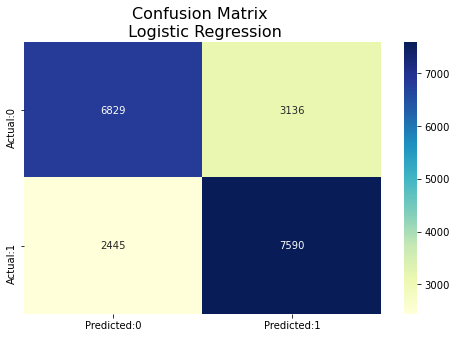
\includegraphics[width=90mm,height=\textheight,keepaspectratio]{images/log_conf_matrix.png}
    \caption{Logistic Regression Confusion Matrix}
    \label{fig:log_conf_matrix}
\end{figure}

\noindent
Using \cref{fig:log_conf_matrix} and Equations \ref{eq:sensitivity}, \ref{eq:specificity}, and \ref{eq:accuracy}, I calculated the sensitivity, specificity, and accuracy of my model.

\begin{align}
    \text{Sensitivity} &= \frac{TP}{TP + FN} \\ \label{eq:sensitivity}
    &= \frac{7590}{7590 + 2445} \\
    &\approx 75.6\% \\
    \text{Specificity} &= \frac{TN}{TN + FP} \\ \label{eq:specificity}
    &= \frac{6829}{6829 + 3136} \\
    &\approx 68.5\% \\
    \text{Accuracy} &= \frac{TP + TN}{TP + FP + FN + TN} \\ \label{eq:accuracy}
    &= \frac{7590 + 6829}{7590 + 3136 + 2445 + 6829} \\
    &\approx 72.1\% 
\end{align}
\noindent
where:
\begin{itemize}
    \item $TP$ is the number of True Positives.
    \item $TN$ is the number of True Negatives.
    \item $FP$ is the number of False Positives.
    \item $FN$ is the number of False Negatives.
\end{itemize}

\noindent
As can be seen in Equations \ref{eq:sensitivity}, \ref{eq:specificity}, and \ref{eq:accuracy}, the model has a relatively low sensitivity, specificity, and accuracy. I believe that a stronger predictive model can be created.

\subsection{Random Forest Classifier}
Given relatively weak results from \cref{section:logistic_regression}, I decided to try the more advanced Random Forest Classifier using GridSearchCV. Random Forest classifier is a machine learning model that combines the predictions of multiple decision trees to make more accurate and robust classifications. It works by creating a forest of decision trees, each trained on a random subset of the data and using a random subset of the features. The individual tree predictions are then aggregated to make the final classification decision, often through a majority vote or weighted average. Random Forests are known for their ability to handle high-dimensional data, reduce overfitting, and provide feature importance rankings, making them a popular choice for a wide range of classification tasks, from image recognition to financial risk assessment.

\subsubsection{Results}
\begin{figure}[H]
    \centering
    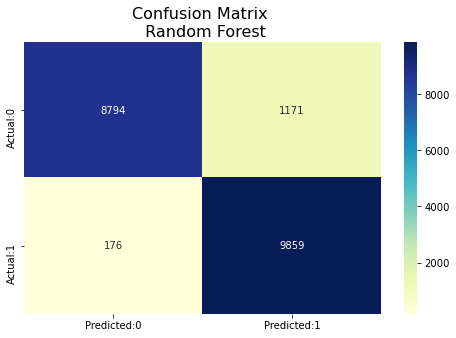
\includegraphics[width=90mm,height=\textheight,keepaspectratio]{images/rf_conf_matrix.png}
    \caption{Random Forest Confusion Matrix}
    \label{fig:rf_conf_matrix}
\end{figure}

\begin{align}
    \text{Sensitivity} &= \frac{TP}{TP + FN} \\ \label{eq:sensitivity2}
    &= \frac{9859}{9859 + 176} \\
    &\approx 98.2\% \\
    \text{Specificity} &= \frac{TN}{TN + FP} \\ \label{eq:specificity2}
    &= \frac{8794}{8794 + 1171} \\
    &\approx 88.2\% \\
    \text{Accuracy} &= \frac{TP + TN}{TP + FP + FN + TN} \\ \label{eq:accuracy2}
    &= \frac{9859 + 8794}{9859 + 1171 + 176 + 8794} \\
    &\approx 93.3\% 
\end{align}

\cref{fig:rf_conf_matrix} and Equations \ref{eq:sensitivity2}, \ref{eq:specificity2}, and \ref{eq:accuracy2} clearly show that the Random Forest Model is more sensitive, specific, and accurate than the Logisitic Model in \cref{section:logistic_regression}. Since the sensitivity (true positive rate) is \(98\%\) and the specificity (true negative rate) is \(88\%\), the Random Forest Classifier seems to miscategorize more non-severe accidents as severe \citep{zhu2010sensitivity}. This is acceptable for the practical application of this model as overestimating the severity of accidents would bring greater public awareness of dangerous driving conditions.